\section{Introduction}

Surface waves form at the free surface of a liquid. For additional clarity, they are sometimes called surface gravity waves. This emphasizes that gravity (and not, for example, surface tension) is the dominant restoring force.

Surface waves have captured the interest of many scientists. Michael Faraday was among them and he was sufficiently successful to have a problem in surface wave motion named after him. In 1831, Faraday reported to the Royal Society \citep{faraday31:_acous_figur} on experiments he did in which a thin layer of water was placed on a vibrating membrane. Faraday established that the standing waves that form on the plate have an oscillation frequency equal to one-half the vertical forcing frequency used to produce them. It is due to this discovery that nowadays, many investigations in wave excitation are known under the rubric of the `Faraday problem.'

% % Faraday's result established 1:2 ratio with external forcing, to
% % produce 1:1 internal resonance, is horizontal forcing required, or
% % is vertical forcing also acceptable? Check paper given by NSN on
% % canonical transformation

In certain applications, for example in experiments carried out on spacecraft where `g-jitter' is hard to eliminate \citep{walter87:_fluid}, there is a need to describe the surface gravity wave patterns that form under the influence of `noisy' forcing. Thus, in the present development we focus on stochastic forcing. Specifically, we examine the long-term evolution of a horizontally excited Faraday system when two wave-modes are near 1:1 resonance and show that in this case, rather than studying the fast timescale evolution of two individual wave modes (i.e. a four-dimensional system), one can focus on the long timescale evolution of two conserved quantities (the Hamiltonian and the angular momentum.)

\section{Surface-Gravity Wave Model}
\subsection{Governing Equations}
\label{s:governing equations}

Although our ultimate goal is to study surface wave patterns, we begin by considering the `internal' motion of the fluid at whose surface these wave patterns form. For an incompressible fluid whose velocity is described by the vector $\boldsymbol{u}$, the Boussinesq approximation~\citep{kundu90:_fluid_mechan} holds and conservation of mass is expressed by the continuity equation
\begin{equation}
\nabla \cdot \boldsymbol{u}= 0 \label{e:Cons Mass}
\end{equation}
For a fluid particle with density $\rho$, pressure $p$ and viscosity $\nu$ (and with gravity represented by the vector $\boldsymbol{g}$), conservation of momentum is expressed by the equation
\begin{equation}
\rho \left[ \frac{\partial \boldsymbol{u}}{\partial t} + (\boldsymbol{u} \cdot \nabla )\boldsymbol{u} \right] = - \nabla p + \rho \boldsymbol{g}+ \nu \nabla^2 \boldsymbol{u}. 
\end{equation}
This equation is known by many as the Navier-Stokes equation. We are working towards a Hamiltonian formulation, therefore we assume the fluid is inviscid and the Navier-Stokes equation simplifies to the Euler equation
\begin{equation}
\rho \left[ \frac{\partial \boldsymbol{u}}{\partial t} + (\boldsymbol{u} \cdot \nabla )\boldsymbol{u} \right] = - \nabla p + \rho \boldsymbol{g}.
\end{equation}
Note, however, that we will reintroduce viscous effects (in \S\ref{s:damping}) in the form of linear damping.

Next, the fluid motion is assumed irrotational: $\nabla \times \boldsymbol{u}= 0$. This assumption can either be introduced ad-hoc, or it can be inferred from Kelvin's circulation theorem. The latter states that for inviscid fluids, rotational motion is conserved. Therefore, if we take the initial state of the fluid to be irrotational, it will remain irrotational forever after. Irrotational fluid motions can be described by a velocity potential $\boldsymbol{u}= \nabla \phi$. The conservation of momentum equation becomes
\begin{equation}
\frac{\partial \phi}{\partial t} + \frac12 |\boldsymbol{u}|^2 + \frac{p}{\rho} + g z = 0.
\end{equation}
In the above, it has been assumed gravity acts along the vertical direction, therefore $|\boldsymbol{g}|=g$.

In order to relate the motion of the surface waves to the internal motion of the fluid, boundary conditions are needed. First, there is the kinematic boundary condition. As explained in \citet{whitham74:_linear}, derivation of this boundary condition, the kinematic boundary condition is based on the surface of the fluid being defined by the property that no fluid crosses it. This surface has height
\begin{equation}
z = \eta (x_1, x_2, t)
\end{equation}
($x_1$ and $x_2$ refer to the coordinates of the horizontal plane, in actual calculations we use cylindrical coordinates, thus $x_1 = r$ and $x_2 = \theta$) and the kinematic boundary condition is given by
\begin{equation}
\frac{\partial \eta}{\partial t} + \nabla \eta \cdot \boldsymbol{u} = u_z \quad \text{at } z = \eta
\end{equation}
In the above, we have made use of the notation $\boldsymbol{u} = (u_{x_1}, u_{x_2}, u_z )$.

In our treatment, we take the fluid to be confined to a cylindrical tank of radius $a$ and depth $d$ (at rest the fluid is contained between $z = -d$ and $z = 0$.) This leads to boundary conditions at the lateral and bottom walls of the tank that state that there is no flow across these walls
\begin{gather*}
u_r = 0 \quad \text{at } r = a\\
u_z = 0 \quad \text{at } z = - d
\end{gather*}

An essential contribution made by \citet{miles76:_nonlin} is to show that the conservation of mass equation, the kinematic boundary condition and the boundary conditions at the lateral and bottom walls can be obtained from a variational formulation. Specifically, the first variation of the integral
\begin{equation}
\begin{split}
SI (\phi)& = \int_{\theta = 0}^{2 \pi} \int_{r = 0}^a \int_{z = - d}^{\eta ( r, \theta, t )} \frac12 | \nabla \phi |^2 dz \, dS - \int_{\theta = 0}^{2 \pi} \int_{r = 0}^a  \phi |_{z = \eta} \frac{\partial \eta}{\partial t} dS
\end{split}
\end{equation}
must vanish ($S = \pi r^2$ is the cross-sectional area of the basin). Miles's derivation was based on work by \citet{serrin59:_encyc_physic}. Note that Miles's derivation is different from the oft-cited variational in \citet{luke67:_variat_princ_for_fluid_with_free_surfac} since the latter also recovers the dynamic boundary condition. Note furthermore that a similar variational analysis was obtained earlier by \citet{zakharov68:_stabil_of_period_waves}.

First, separation of variables is used to write
\begin{align*}
\eta (x_1,x_2, t)& = q_n (t) \psi_n (x_1,x_2),\\
\phi (x_1,x_2,z,t)& = \phi_n (t) \chi_n (x_1,x_2,z).
\end{align*}
The relationship between $\psi_n$ and $\chi_n$ is found from the conservation of mass equation, the boundary condition at the container's walls and a linearization of the kinematic boundary condition
\begin{equation}
\frac{\partial \eta}{\partial t} = \frac{\partial \phi}{\partial z} \quad \text{at } z = 0.
\end{equation}
The relation between $\phi_n(t)$ and $q_n(t)$ is found using the variational formulation. Details are given in~\citet[\S2]{miles76:_nonlin}.

% Give specific form of eigenfunctions, and eigenvalues for
% cylindrical geometry

% Show sample diagram of surface wave pattern

\subsection{The Hamiltonian of Surface-Gravity Waves}
\label{s:Hamiltonian}

Stochastic averaging may be seen as a procedure used to reduce the number of dimensions of a system. The lower-dimensional system's long-term evolution is given in terms of quantities that are constants of motion of the original (higher dimension) system over short timespan. This motivates our interest in determining the Hamiltonian for the surface-gravity wave system. First, we write expressions for the kinetic and potential energies. These give the Lagrangian from which the Hamiltonian follows.

The kinetic energy is
\begin{eqnarray*}
T & = & \frac12 \int | \nabla \phi |^2 dS dz\\
& = & \frac{\rho S}{2} a_{mn} \dot{q}_m \dot{q}_n .
\end{eqnarray*}
The second form of $T$ makes use of the results in~\citet{miles76:_nonlin}, where it is shown that
\begin{equation}
a_{mn} = \delta_{mn} a_m + a_{lmn} q_l + \frac12 a_{jlmn} q_j q_l + O ( q^2 )
\end{equation}
The quantities $a_{lmn}$ and $a_{jlmn}$ are constants. The potential energy of the free-surface, displaced from its equilibrium position, is
\begin{eqnarray}
V &=& \rho \int dS \int^{\eta}_{z = 0} |\boldsymbol{g}| z dz \label{e:potential energy}\\
&=& \frac{\rho S}{2} g q_n q_n. \nonumber
\end{eqnarray}
The Lagrangian, which for convenience we normalize by $\rho S$, is
\begin{eqnarray*}
L &=& \frac{1}{\rho S} ( T - V )\\
& = & \frac12 ( a_{mn} \dot{q}_m \dot{q}_n - g q_n q_n ) .
\end{eqnarray*}
and the Hamiltonian is
\begin{equation}
\label{e:Hamiltonian}
H = \frac12 (h_{mn}(q) p_m p_n + g q_n q_n).
\end{equation}
Note that this Hamiltonian contains quadratic terms, but also higher order terms since the coefficient $h_{mn}$ depends on $q_n$
\begin{equation}
\label{e:hamiltonian coefficient expansion}
h_{mn} = \delta_{mn} \frac{\omega_m^2}{g} + h_{lmn} q_l + \frac12 h_{jlmn} q_j q_l + O(q^3).
\end{equation}
The equations for $h_{lmn}$ and $h_{jlmn}$ are given in \citet{miles76:_nonlin} and reproduced in Appendix~\ref{a:non-linear Hamiltonian}

\subsection{Damping and Forcing Effects}
\label{s:damping}

We are interested in the effects of stochastic forcing. To balance forcing effects, damping is necessary. Physically, damping stems from the viscosity of the fluid, but for simplicity we introduce damping ad-hoc. We use linear damping coefficients, $\alpha_k$ to supplement the momentum equation.
% FIXME This approach is also used by Miles in \cite{miles84:_inter}, however Miles also supplements the equations for $q_1$ and $q_2$ with damping, but it is not clear how to physically justify the damping of coordinates.

To account for forcing effects, we follow the method presented in~\citet{miles76:_nonlin}. Terms are added to the potential energy given in Equation (\ref{e:potential energy}), thus
% FIXME Should not have to give multiple references to miles76:_nonlin
\begin{equation}
\begin{split}
V &= \rho \int dS \int^{\eta}_{z = 0} \bigl[ \dot{\xi}_{x_1}
x_1 + \dot{\xi}_{x_2} x_2 + (g + \dot{\xi}_z) z \bigr] dz\\
&= \rho S \bigl( - Q_n q_n + \frac12 (g + \dot{\xi}_z) q_n q_n
\bigr)\label{e:V with forcing}.
\end{split}
\end{equation}
In the above $\xi_{x_1}$ and $\xi_{x_2}$ specify the imposed horizontal velocities of the tank while $\xi_z$ is the vertical velocity and
\begin{align}
Q_n & = - \dot{\xi}_{x_1} x_{1 n} - \dot{\xi}_{x_2} x_{2
n}\\ x_{1 n} & \equiv S^{- 1} \int x_1 \psi_n dS\label{e:SI def}\\ x_{2 n} &
\equiv S^{- 1} \int x_2 \psi_n dS
\end{align}
With forcing and damping, the equations governing the motion of the
surface-gravity waves are, for $t\geq0$,
\begin{align}
\dot{q}_k &= \frac{\partial H}{\partial p_k}\\
\dot{p}_k &= -\frac{\partial H}{\partial q_k} + \alpha_k p_k +
\dot{\xi}_z q_1 + \dot{\xi}_{x_1} x_{1k} + \dot{\xi}_{x_2} x_{2k}
\end{align}

\section{Stochastic Analysis}
In this section, we analyze the equations of motion presented in the
previous section under the influence of stochastic
forcing. Specifically, we concentrate on the motion of two wave modes
near resonance.

\subsection{Integrals of Motion}\label{s:Integrals of motion} In
order to study the effects of small amplitude noise over long time
scales, we introduce a small scaling parameter $\epsilon$
($0<\epsilon\ll1$.) First, we rescale the canonical variables by
$\sqrt{\epsilon}$
\begin{align*}
q &=\sqrt{\epsilon}\tilde{q}& 
p &=\sqrt{\epsilon}\tilde{p}.
\end{align*}
Concentrating our analysis on the two wave modes (near resonance), we use the canonical transformation
\begin{gather*}
\tilde{q}_{1,2} = x_{1,2} \cos \omega_{1,2} t +\tfrac{\omega_{1,2}}{g} y_{1,2} \sin
\omega_{1,2} t\\
\tilde{p}_{1,2} = -\tfrac{g}{\omega_{1,2}} x_{1,2} \sin \omega_{1,2} t + y_{1,2} \cos
\omega_{1,2} t
\end{gather*}
% FIXME \omega vs. omega_{1,2} and \epsilon
This transformation eliminates terms of order $\epsilon$ in the
Hamiltonian. The lowest order terms of the Hamiltonian are now of
order $\epsilon^{3/2}$. Terms of that order are eliminated by
setting the two wave modes near resonance with one another, so that
$\omega_{1,2} = \omega + \epsilon \sigma_{1,2}$. This imposition and the time averaging operator from Definition \ref{d:Tave} eliminate terms of order $\epsilon^{3/2}$ from the Hamiltonian. Thus the dynamics of the system acquire the form
\begin{align}
\dot{\boldsymbol{x}}^{\epsilon}_t& = \epsilon \boldsymbol{b}^1
(\boldsymbol{x}^{\epsilon}_t,t) + \epsilon^2 \boldsymbol{b}^2
(\boldsymbol{x}^{\epsilon}_t,t) + \epsilon \boldsymbol{g}
(\boldsymbol{x}^{\epsilon}_t,t)
\label{e:standard form}
\end{align}
% \begin{equation}
% \boldsymbol{b}^1 \equiv \frac{1}{\epsilon^2} \bar{\nabla} H, \quad
% \bar{\nabla} \equiv
% \Bigl(
% \frac{\partial}{\partial y_1}, 
% -\frac{\partial}{\partial x_1},
% \frac{\partial}{\partial y_2},
% -\frac{\partial}{\partial x_2}
% \Bigr)
% \end{equation}
% is of order 1 in $\epsilon$ and corresponds to the `Hamiltonian
% dynamics' term in the equation
% \begin{align}
% \dot{\boldsymbol{x}}^{\epsilon}_t& = \epsilon \boldsymbol{b}^1
% (\boldsymbol{x}^{\epsilon}_t,t) + \epsilon^2 \boldsymbol{b}^2
% (\boldsymbol{x}^{\epsilon}_t,t) + \epsilon \boldsymbol{g}
% (\boldsymbol{x}^{\epsilon}_t,t), & t \geq 0 \label{e:standard form}\\
% \boldsymbol{x}_0^\epsilon& = \boldsymbol{x}\nonumber \in \R^4
% \end{align}
% $\boldsymbol{b}^2$ refers to damping terms
% \begin{align*}
% \boldsymbol{b}^2 \equiv
% \Bigl(&
% \frac{\omega}{g} \alpha_1  \left[ -\frac{g}{\omega} x_1 \sin
% \omega t + y_1 \cos \omega t \right] \sin \omega t
% ,\\&
% \alpha_1 [-\frac{g}{\omega} x_1 \sin \omega t + y_1 \cos
% \omega t] \cos \omega t
% ,\\&
% \frac{\omega}{g} \alpha_2  \left[-\frac{g}{\omega} x_2
% \sin \omega t + y_2 \cos \omega t \right] \sin \omega t
% ,\\&
%  \alpha_2 [ - \frac{g}{\omega} x_2 \sin \omega t + y_2 \cos
% \omega t] \cos \omega t
% \Bigr)
% \end{align*}
% $\boldsymbol{g}$ contains stochastic forcing terms. Note that because
% vertical forcing is parametric whereas horizontal forcing is additive,
% if one were interested in a problem with both types of forcing
% present, the horizontal forcing would need to be smaller than the
% vertical forcing by a factor of $\sqrt{\epsilon}$, as can be seen from
% Equation~\eqref{e:V with forcing}. We avoid this complication by
% considering only horizontal forcing.
% \begin{align*}\label{e:g def}
% \boldsymbol{g} \equiv
% \Bigl(&
% \frac{\omega}{g} \Bigl[ \dot{\xi}_z \Bigl( x_1 \cos \omega t +
% \frac{\omega}{g} y_1 \sin \omega t \Bigr) + \dot{\xi}_{x_1} x_{11}
% + \dot{\xi}_{x_2} x_{21} \Bigr]  \sin \omega t
% ,\\ &
% \frac{\omega}{g} \Bigl[\dot{\xi}_z \Bigl( x_1 \cos \omega t +
% \frac{\omega}{g} y_1 \sin \omega t \Bigr) + \dot{\xi}_{x_1} x_{11}
%  + \dot{\xi}_{x_2} x_{21} \Bigr] \cos \omega t
% ,\\ &
% \frac{\omega}{g}  \Bigl[ \dot{\xi}_z \Bigl( x_2 \cos \omega t +
% \frac{\omega}{g} y_2 \sin \omega t \Bigr) + \dot{\xi}_{x_1} x_{12}
%  + \dot{\xi}_{x_2} x_{22} \Bigr] \sin \omega t
% ,\\ &
% \frac{\omega}{g} \Bigl[
% \dot{\xi}_z \Bigl( x_2 \cos \omega t + \frac{\omega}{g} y_2 \sin \omega t
% \Bigr) + \dot{\xi}_{x_1} x_{12} 
%  + \dot{\xi}_{x_2} x_{22} \Bigr] \cos \omega t
% \Bigr)
% \end{align*}
Equation~\eqref{e:standard form} is helpful in showing
the three timescales present in this problem. Owing to their small
amplitude (i.e. $\epsilon^2$), the effects of noise and damping have an
influence only over long times, of order $1/\epsilon^2$. The
Hamiltonian dynamics, associated with the components of
$\boldsymbol{b}^1$ are of order $\epsilon$, thus they fluctuate over a
faster timescale, of order $1/\epsilon$. Finally, the fastest
fluctuations occur due periodicity of some of the coefficients that
constitute $\boldsymbol{b}^1$. The coefficients fluctuate over a
period $\omega/2\pi$, which is of order 1. % Our interest is primarily
% in the influence of stochastic forcing, thus we must use two averaging
% steps, the first to average the periodic coefficients and the second
% to average the dynamics of $\boldsymbol{b}^1$. This type of stochastic
% averaging was developed in Namachchivaya and
% Sowers~\cite{namachchivaya01:_unified_approac_noisy_nonlin_mathieu_type_system}
% for a two-dimensional system. Here we apply the method to a
% four-dimensional system, following the extensions presented
% in~\cite{namachchivaya:_random}.

% In order for a four-dimensional system to be integrable, two integrals
% of motion are needed. To find these constants, we begin by defining
% our first averaging operator. For a function $\varphi$ that is
% time-periodic with period $\omega/2 \pi$
% \begin{equation}
% \Tave\varphi \equiv \frac{\omega}{2\pi}
% \int_0^{2\tfrac{\pi}{\omega}} \varphi(t) dt
% \label{e:time averaging defn}
% \end{equation}
% This is a deterministic averaging operator. Applying this
% operator to the periodic coefficients (those that fluctuate over
% timescales of order 1) eliminates them, so that the fastest timescale
% of the problem is now of order $1/\epsilon$.
We rescale time such that leading order dynamics become of order
1. If $\tilde{\boldsymbol{x}}_t^{\epsilon} \equiv
\boldsymbol{x}_{t/\epsilon}^{\epsilon}$. Equation~\eqref{e:standard
form} becomes
\begin{align*}
\dot{\tilde{\boldsymbol{x}}}^{\epsilon}_t& = \boldsymbol{b}^1
({\tilde{\boldsymbol{x}}}^{\epsilon}_t,t/\epsilon) + \epsilon
\boldsymbol{b}^2
({\tilde{\boldsymbol{x}}}^{\epsilon}_t,t/\epsilon) +
\boldsymbol{g} (\tilde{\boldsymbol{x}}^{\epsilon}_t,t/\epsilon)
\end{align*}
% \begin{align*}
% \dot{\tilde{\boldsymbol{x}}}^{\epsilon}_t& = \boldsymbol{b}^1
% ({\tilde{\boldsymbol{x}}}^{\epsilon}_t,t/\epsilon) + \epsilon
% \boldsymbol{b}^2
% ({\tilde{\boldsymbol{x}}}^{\epsilon}_t,t/\epsilon) +
% \boldsymbol{g} (\tilde{\boldsymbol{x}}^{\epsilon}_t,t/\epsilon), & t
% &\geq 0\\
% \tilde{\boldsymbol{x}}_0^\epsilon& = \boldsymbol{x} \in \R^4
% \end{align*}
With the equation in this form, we are able to apply a result from~\citet{khas'minskii66:_stoch_proc}. This result tells us that as $\epsilon \to 0$, $\tilde{\boldsymbol{x}}_t^\epsilon$ converges in probability to
\begin{align*}
\dot{\boldsymbol{x}}_t &= \Tave[\boldsymbol{b}^1(\boldsymbol{x}_t,t/\epsilon)] = \bar{\nabla}\Tave[H(\boldsymbol{x}_t)] = \bar{\nabla} K(\boldsymbol{x}_t), & t \geq 0\\
\boldsymbol{x}_0 &= \boldsymbol x \in \reals^4
\end{align*}
The averaged Hamiltonian, $K$, is our first integral of motion.
\begin{multline*}
K =\frac{1}{192 g^3 \omega}\bigl[3 k^2 K_1 (y_1^2+y_2^2)^2
\omega^5 + 3g^4 (32(\sigma_1 x_1^2 + \sigma_2 x_2^2)+k^2 K_1 \omega
(x_1^2+x_2^2)^2)\\
+ 2g^2 \omega^2 \{48(\sigma_1 y_1^2 + \sigma_2 y_2^2) + k^2 (32 K_{-1}
(x_2 y_1-x_1 y_2)^2+K_1[(3 x_1^2+x_2^2) y_1^2 \\
+ 4 x_1 x_2 y_1 y_2 + (x_1^2 + 3 x_2^2) y_2^2])\omega\}\bigr]
\end{multline*}

% In Mathematica file, K = H - O(2) terms

% In order to find the second integral of motion, we take advantage of
% the fact we are interested in 1:1 resonance by writing
% $\omega_1=\omega + \epsilon \sigma_1$ and $\omega_2=\omega + \epsilon
% \sigma_2$. This introduces `detuning', of order $\epsilon$ into the
% problem. Note that we have the freedom to choose the order of the
% detuning; detuning of order $\epsilon$ is chosen so that detuning is
% of the same order as the Hamiltonian terms that do not vanish under
% time-averaging. Detuning could be made of higher-order, in which case
% its effects would presumably be chosen to be of the same order as
% stochastic forcing and damping. Setting $\omega_1$ and $\omega_2$ as
% stated provides a second integral of motion:

The second integral of motion will be denoted by $I$ and represents
angular momentum.
\begin{equation}
I= \frac{1}{2 g \omega}\bigl[g^2(x_1^2+x_2^2)+\omega^2(y_1^2+y_2^2)\bigr].
\end{equation}

\subsection{Structure of the Unperturbed System}
\label{s:unperturbed structure}

As stated in the previous section, the surface wave system in 1:1 resonance has two constants of motion, $K$ and $I$. We now introduce a canonical transformation that takes advantage of this fact by making the angular momentum one of the canonical variables. The canonical transformation from $(x_1,y_1,x_2,y_2)$ to $(X,Y,\theta,I)$ is given by
\begin{align*}
x_1& = \frac{\sqrt{\frac{\omega}{g}(X^2+Y^2)}}{Y \sqrt{1+\frac{X^2}{Y^2}}} (Y \cos \theta - X \sin \theta)\\
y_1& = -\frac{\sqrt{\frac{g}{\omega}(X^2+Y^2)}}{Y \sqrt{1+\frac{X^2}{Y^2}}} (X \cos \theta + Y \sin \theta)\\
x_2& = \sqrt{\frac{\omega}{g} (2I-X^2-Y^2)} \cos \theta\\
y_2& = -\sqrt{\frac{g}{\omega} (2I-X^2-Y^2)} \sin \theta.
\end{align*}
Introducing the variables
\begin{align*}
\alpha &\equiv \frac{k^2 \omega^2}{24 g}(K_1 - 16 K_{-1}) & \beta 
&\equiv \frac{3 k^2 \omega^2}{24 g} K_1
\end{align*}
the averaged Hamiltonian is
\begin{equation}
\label{e:averaged K}
K = \frac{\alpha}{2} (X^2 + Y^2 - 2 I) X^2 + \frac{\beta}{2} I^2 + \frac{\sigma_1 - \sigma_2}{2}(X^2 + Y^2) + \sigma_2 I
\end{equation}
and the equations of motion are
\begin{equation}
\label{e:sgwaves fast planar}
\begin{gathered}
\dot{X}_t = (\alpha X_t^2 + \sigma_1 - \sigma_2) Y_t\\
\dot{Y}_t = [\alpha(2I_t - 2X_t^2 - Y_t^2) - \sigma_1 + \sigma_2] X_t\\
\dot I_t = 0\\
\dot \theta_t = \beta I_t - \alpha X_t^2 + \sigma_2
\end{gathered}
\end{equation}
% FIXME Add order epsilon terms to these equations
This canonical transformation decouples the equations
for $X_t$ and $Y_t$ from those for $\theta_t$, and, consistent with
the results of \S\ref{s:Integrals of motion}, $I_t$ is a
constant (effectively a parameter) since $\dot{I}_t=0$. $I$ acts as a
bifurcation parameter. Defining the critical value
\begin{equation}
I_c = \frac{\sigma_1 - \sigma_2}{2 \alpha},
\end{equation}
when $I<I_c$ phase portraits in the $X,Y$ plane have a single elliptic
fixed point at the origin. For $I>I_c$, the fixed point at the origin
becomes a saddle point and two fixed points on the $X$ axis
appear. The coordinates of these fixed points are
\begin{align}
X &= \pm \sqrt{I + \frac{\sigma_2 - \sigma_1}{2 \alpha}} &
Y = 0
\end{align}

% This is depicted in Figure~\ref{f:bifurcation and phase portrait}.

The stochastic diffusion process that we will study is described in terms of the variables $K$ and $I$. The $K-I$ domain is shown in figure~\ref{f:HI domain}. In that figure, $I$ ranges from 0 to 0.5, but the upper limit can be made arbitrarily large. The range of $K$ is not arbitrary. The maximum value, $K_e$ occurs at the elliptic fixed points. There is also a minimum value, $K_{2I}$, since the canonical transformation introduces the restriction $X^2 + Y^2 \leq 2 I$. Note that the domain between $K_s$ and $K_e$ exits for both elliptic fixed points, thus, the entire $K-I$ domain may be described as a three-leaved open-book, a nomenclature used in~\citet{freidlin04:_diffus}, or an arrowhead.

% FIXME State that a cusp exists in the domain.

% \begin{figure}
% \begin{center}
% \includegraphics[width=\textwidth*5/8,angle=-90]{../../matlab/figures/phaseportrait_xy_3d_subcrit}
% \caption{Phase-space portrait in the $X,Y$ plane when $I < I_c$}
% \label{f:X Y phase portrait I < I_c}
% \end{center}
% \end{figure}

% \begin{figure}
% \begin{center}
% \includegraphics[width=\textwidth]{../../matlab/figures/phaseportrait_xy_3d_supcrit}
% \caption{Phase-space portrait in the $X,Y$ plane when $I > I_c$}
% \label{f:X Y phase portrait}
% \end{center}
% \end{figure}

% FIXME Produce and insert figure below
% \begin{figure}
% \begin{center}
% \includegraphics[width=\textwidth]{figures/bifurcation_and_phase_portrait}
% \caption{Phase-space portrait and bifurcation diagram}
% \label{f:bifurcation and phase portrait}
% \end{center}
% \end{figure}

\begin{figure}
\begin{center}
\psfrag{x}{$K$}
\psfrag{y}{$I$}
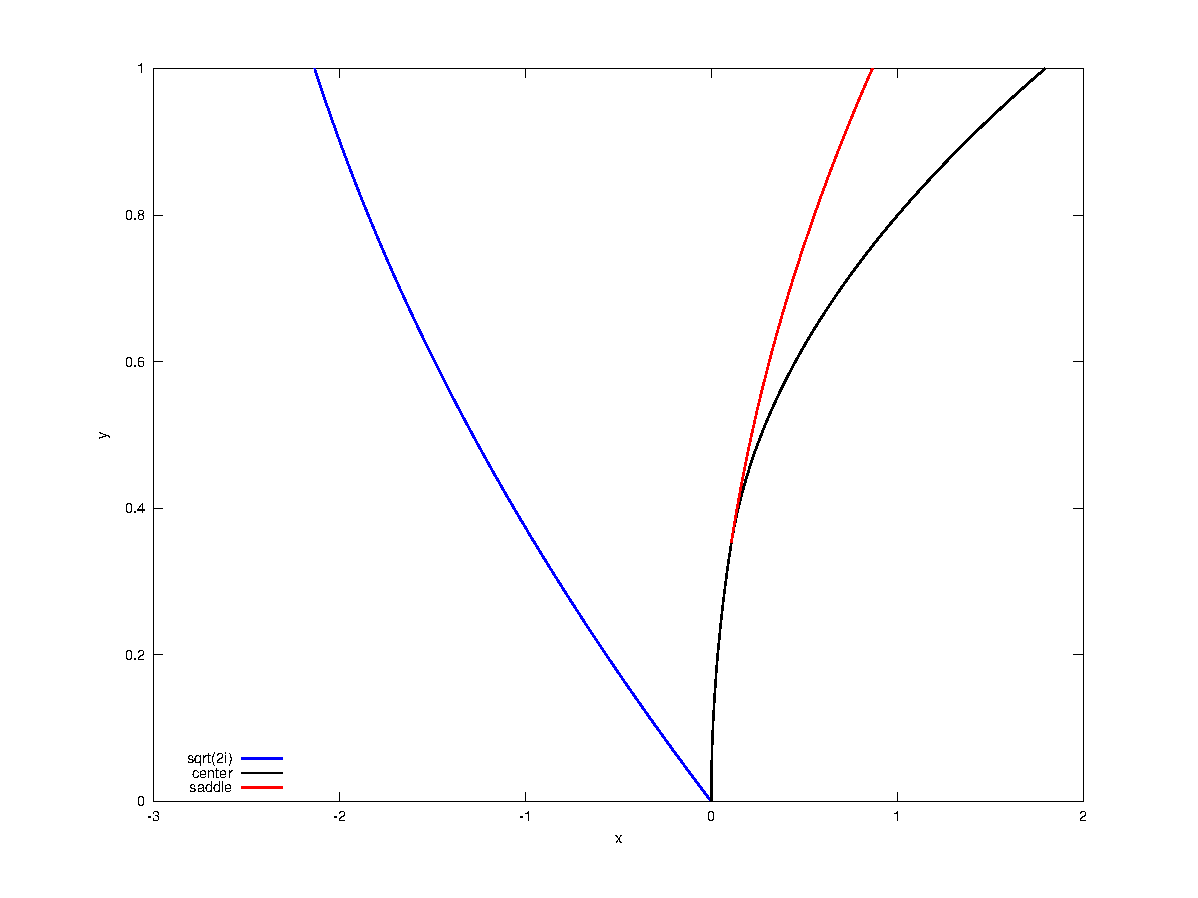
\includegraphics[width=\textwidth*7/8,angle=0]{figures/HIdomain}
\caption{$K-I$ domain}
\label{f:HI domain}
\end{center}
\end{figure}
% FIXME Add FEM triangulation to this figure

% \subsection{Evolution of the Integrals of Motion}

% The ultimate goal of our analysis is to understand the effects of noise. The amplitude of the noise being small, its effects are seen only over long times. The effect of noise (and damping) is seen in the evolution of the two conserved quantities, $K$ and $I$. It seems natural therefore, to define the map $\mathcal{Y}: \reals^4 \to \reals^2$ by
% \begin{equation}
% \mathcal{Y}(\boldsymbol{x}) \equiv (K(\boldsymbol{x}),I(\boldsymbol{x})), \qquad \boldsymbol{x}\in \reals^4.
% \end{equation}
% Since $\lim_{\epsilon \to 0}\boldsymbol{x}^\epsilon_t =
% \boldsymbol{x}_t$,
% % Need to quote Khasminksii here?
% \begin{equation}
% \lim_{\epsilon \to 0}(K(\boldsymbol{x}^\epsilon_t),I(\boldsymbol{x}^\epsilon_t)) = (K(\boldsymbol{x}_t),I(\boldsymbol{x}_t)).
% \end{equation}
% The evolution of $\boldsymbol{y}^{\epsilon}_t \equiv \mathcal{Y}(\boldsymbol{x}^{\epsilon}_t )$ is given by
% \begin{align}
% \dot{\boldsymbol{y}}^{\epsilon}_t& = \epsilon F^1(\boldsymbol{x}^{\epsilon}_t,t) + \epsilon^2 F^2(\boldsymbol{x}^{\epsilon}_t,t) + \epsilon G
% (\boldsymbol{x}^{\epsilon}_t,t), & t& \geq 0 \label{e:SDE}\\
% \boldsymbol{y}_0^\epsilon& = (K(\boldsymbol{x}),I(\boldsymbol{x}))
% \end{align}
% where
% \begin{align*}
% F^1_1& = \sum^4_{i = 1} \frac{\partial K}{\partial\boldsymbol{x}_i} \boldsymbol{b}^1_i&
% F^1_2& = \sum^4_{i = 1} \frac{\partial I}{\partial\boldsymbol{x}_i} \boldsymbol{b}^1_i\\
% F^2_1& = \sum^4_{i = 1} \frac{\partial K}{\partial\boldsymbol{x}_i} \boldsymbol{b}^2_i&
% F^2_2& = \sum^4_{i = 1} \frac{\partial I}{\partial\boldsymbol{x}_i} \boldsymbol{b}^2_i\\
% G_1& = \sum^4_{i = 1} \frac{\partial K}{\partial\boldsymbol{x}_i} \boldsymbol{g}_i&
% G_2& = \sum^4_{i = 1} \frac{\partial I}{\partial \boldsymbol{x}_i} \boldsymbol{g}_i
% \end{align*}
% Since $K$ and $I$ are integrals of motion, $\Tave F^1 (\boldsymbol{x}) = 0$. Thus, to see the fluctuations of $K$ and $I$, we need to look on an a timescales of order $1/\epsilon^2$. Thus, we rescale time again, setting $\boldsymbol{X}^{\epsilon}_t \equiv \boldsymbol{x}^{\epsilon}_{t / \epsilon^2}$ and $\boldsymbol{Y}_t^{\epsilon} \equiv \boldsymbol{y}^{\epsilon}_{t / \epsilon^2}$. This yields
% \begin{align}
% \dot{\boldsymbol{X}}^{\epsilon}_t& = \frac{1}{\epsilon} b^1 (
% \boldsymbol{X}^{\epsilon}_t, t/\epsilon^2) + b^2
% (\boldsymbol{X}^{\epsilon}_t,t/\epsilon^2) + \frac{1}{\epsilon}
% g(\boldsymbol{X}^{\epsilon}_t,t/\epsilon^2), & \label{e:X}
% t&\geq 0\\
% \boldsymbol{X}^\epsilon_0& = \boldsymbol{x} \in \reals^4 \nonumber
% \end{align}
% \begin{align}
% \dot{\boldsymbol{Y}}^{\epsilon}_t& = \frac{1}{\epsilon} F^1
% (\boldsymbol{X}^{\epsilon}_t,t/\epsilon^2) + F^2
% (\boldsymbol{X}^{\epsilon}_t,t/\epsilon^2) + \frac{1}{\epsilon}
% G(\boldsymbol{X}^{\epsilon}_t,t/\epsilon^2), & \label{e:Y}
% t& \geq 0\\
% \boldsymbol{Y}_0^\epsilon& =
% (K(\boldsymbol{x}),I(\boldsymbol{x})) \nonumber
% \end{align}
% FIXME Show that as \eps \to 0, evolution of slow variables becomes independent of fast variables. 

% \subsection{Martingale Problem}

% In order to carry out our stochastic analysis, we must rigorously characterize the dynamics of Equation~\eqref{e:Y}. The classical analysis of such equations dates back to Khas'minksii. As shown in \S\ref{s:unperturbed structure}, the reduced domain (i.e. $K \times I$) of the surface wave equations contains a saddle fixed point. For such a case, as opposed to a domain free of fixed points in its interior, showing that $Y_t^\epsilon$ is a Markov process (where it must be stressed that by this we mean $Y_t^\epsilon$ alone, without being coupled to the $X_t^\epsilon$ equations) has only been done via the martingale problem approach.

% To introduce the martingale problem, let us consider the process $X_t^\epsilon$ rather than $Y_t^\epsilon$. The martingale problem is stated in terms of a canonical process $X_t$. This canonical process is made of deterministic parts (the Hamiltonian dynamics and the damping in our case) and stochastic parts (forcing.) The stochastic part has a probility measure $\mathbbm{P}^o$ and this is also the `induced' probability for $X_t^\epsilon$. $X_t$ on the other hand has a probability measure $\mathbbm{P}^\epsilon$ and the correspondence between the two probability measure is given, in terms of a set $A$, as
% \begin{equation}
% \mathbbm{P}^\epsilon(A) \equiv \mathbbm{P}\{X^\epsilon \in A\}
% \end{equation}
% (this transfers the dependence on $\epsilon$ from the process to the
% measure.)

% The martingale problem states that the measure $\mathbbm{P}^\epsilon$
% is unique and that it has a martingale associated with it. A
% martingale, $M_s$ is a process for which
% \begin{equation}
% \Expectation[M_s | \mathcal{M}_t] = M_t \quad\text{for all }s \ge t.
% \end{equation}
% $\mathcal{M}_t,t\ge 0$ is a filtration.

% The process $Y_t^\epsilon$ `lives' in a reduced 2-D space. Denoting
% the reduced-space canonical process corresponding to $Y_t^\epsilon$ by
% $X_t^\dagger$ and the probability measure of $X_t^\dagger$ by
% \begin{equation}
% \mathbbm{P}^{\epsilon,\dagger}(A) \equiv \mathbbm{P}^\epsilon(Y \in A)
% \quad A \in \mathcal{B}(C[0,\infty),K\times I),
% \end{equation}
% the novel requirements for the class of problems within which the
% stochastic analysis of the surface waves falls is to show the
% existence of the limit
% \begin{equation}
% \mathbbm{P}^\dagger \equiv \lim_{\epsilon \to 0}
% \mathbbm{P}^{\epsilon,\dagger}
% \end{equation}
% % We do not show this proof here (it is in preparation by~\citet{namachchivaya:_random}.) Here we simply emphasize that in order to treat a domain $K \times I$ with fixed points, the Martingale problem approach is required and using this approach, classical results are augmented with gluing conditions.

% \subsection{Generator of the Reduced Markov Process}
% \label{s:MP generator}

% In the previous section, we stated the existence of a reduced process $X_t^\dagger$ with a probability measure $\mathbbm{P}^\dagger$. In this section, we give detailed results characterizing the Markov process.

% Let's denote by $\mathfrak{G} = K \times I$ the space shown in figure~\ref{f:HI domain}. To begin, we decompose $\mathfrak{G}$ into three disjoint regions: one for each of the two regions enclosed by a homoclinic orbit and the third outside the homoclinic orbit.

% %As $\epsilon \to 0$, the dynamics of
% %$\boldsymbol{Y}^{\epsilon}_t$ tend to a two-dimensional Markov
% %process~\cite{NamachchivayaUnpublished}. We turn our attention to
% %finding the generator of this Markov process.

% %For $I<I_c$, the stochastic process evolves in a 2-dimensional
% %plane. In this case, the stochastic averaging results
% %in~\cite{khas'minskii68:_ito} hold, making the our analysis relatively
% %straightforward. As shown in Figure~\ref{f:HI domain},
% %$K$ ranges from its value at $X^2 + Y^2 = 2 I$, which we
% %denote by $K_{2I}$ to its value at the elliptic fixed
% %points, $K_e$ and $I$ ranges from 0 to $I_c$. We denote the
% %space of the averaged system by

% %\begin{equation}
% %\mathfrak{G}=([K_{2I},K_e],[0,I_c])=([\boldsymbol{y}_*,\boldsymbol{y}^*]).
% %\]

% %The generator is
% %% What is the limit y' -> y ? Closure of spaces...
% %\begin{equation}\label{e:generator line process}
% %\begin{split}
% %(\gen_\mathfrak{G}^\dagger f)(\boldsymbol{y})& = \lim_{\boldsymbol{y}'
% %\to \boldsymbol{y}, \boldsymbol{y} \in \mathfrak{G}} (\gen f) (\boldsymbol{y}')\\
% %& = \mathfrak{b}_j(\boldsymbol{y}) \frac{\partial
% %f(\boldsymbol{y})}{\partial \boldsymbol{y}_j} + \frac12
% %\mathfrak{a}_{jk}(\boldsymbol{y}) \frac{\partial^2
% %f(\boldsymbol{y})}{\partial \boldsymbol{y}_j \partial \boldsymbol{y}_k}
% %\end{split}
% %\end{equation}
% %and the domain of the generator is
% %% What BC to apply at I_c boundary?
% %\begin{equation*}
% %\mathfrak{D}_\mathfrak{G}^\dagger = \{f \in C^2(\mathfrak{G}): \lim_{\boldsymbol{y}
% %\to (K_{2I},I)} (\gen f)(\boldsymbol{y}) \text{ exists, }
% %\lim_{\boldsymbol{y}
% %\to (K_e,I)} (\gen f)(\boldsymbol{y}) \text{ exists }
% %\text{ and }\\
% % \lim_{\boldsymbol{y} \to (K,I_c)}(\genf)(\boldsymbol{y})=0\}
% %\end{equation*}
% %The drift coefficient $\mathfrak{b}_i$ and diffusion coefficient
% %$\mathfrak{a}_{ij}$ will be defined shortly (viz. Equations~\eqref{eq:
% %drift coeff} and~\eqref{e:diff coeff}.)

% %When $I>I_c$, the analysis is slightly more involved. To begin, the
% %space $\mathfrak{G}$ is decomposed into three disjoint regions, one
% %inside each of the two homoclinic orbits and the third outside the
% %homoclinic orbits. Thus
% \begin{equation}
% \mathfrak{G} \equiv \bigcup_{i=1}^3 \bar{\mathcal{I}}_i.
% \end{equation}
% Within each $\bar{\mathcal{I}}_i$, we use classical results
% (e.g.~\citet{khas'minskii68:_ito}) to state that the generator of
% the reduced Markov process is, for a function $f \in
% C^2(\reals^2)$,
% \begin{equation} (\gen_{\mathcal{I}_i}^\dagger f)(\bm{y}) = \sum_{j=1}^2
% \mathfrak{b}^i_{y_j}(\bm{y}) \frac{\partial f(\bm{y})}{\partial y_j} +
% \frac12 \sum_{j,k = 1}^2 \mathfrak{a}^i_{y_j y_k}(\bm{y})
% \frac{\partial^2 f(\bm{y})}{\partial y_j \partial y_k}
% \end{equation}
% $\mathfrak{b}$ is the drift coefficient and $\mathfrak{a}$ the diffusion coefficient. In the present problem, because the equations of motion involve time-derivatives of noise, we apply a `real' noise with a specified spectral density rather than white noise (since the latter cannot be differentiated.) % Applying results from \citet{khas'minskii66:_limit_theor} yields the following
% % \begin{align}
% % \mathfrak{b}_{y_i} (\bm{y})& \equiv
% % (\mathbf{A}(\Tave(F^2_i +\mathfrak{g}_i))) (\bm{y})\label{e:drift coeff}\\
% % \mathfrak{a}_{y_j y_k} (\bm{y})& \equiv (\mathbf{A}(\Tave(\sigma\sigma^T)_{jk}))(\bm{y})\label{e:diff coeff}
% % \end{align}
% % where
% % \begin{align}
% % \mathfrak{g}_i& \equiv \int_{-\infty}^0 \Expectation\Bigl[\frac{\partial G_i}{\partial x_j}(\bm{x},t,\xi_t)G_j(\bm{x},t+\tau,\xi_{t+\tau})\Bigr] d\tau \label{e:script g}\\
% % (\sigma\sigma^T)_{jk}& \equiv \int_{-\infty}^\infty \Expectation \Bigl[G_j(\bm{x},t,\xi_t) G_k (\bm{x},t+\tau, \xi_{t+\tau}) \Bigr] d\tau \label{e:sigma sigmat}
% % \end{align}

Note that second order averaging terms have not been included because they may change our results quantitatively but not qualitatively. The small increase in the accuracy of our results is unlikely to be worth the extra effort due to significantly more complex algebraic manipulations.

% $\Aave$ is a spatial averaging operator. It is applied along orbits $S$ on which $K$ and $I$ are constant
% \begin{equation}
% \Aave(\varphi(\bm{y})) \equiv \frac{\int_S \varphi (\bm{y}) \| \bar{\nabla} K(\bm{y})\|^{-1} dS}{\int_S \| \bar{\nabla} K(\bm{y})\|^{-1} dS}.
% \label{e:A averaging}
% \end{equation}
% $\| \bar{\nabla} K(\bm{y})\|$ is a measure of speed,
% thus the denominator corresponds to a period, $\mathcal{T}$. At fixed
% points and on the homoclinic orbit, velocity is zero, thus the
% definition above does not hold. On the homoclinic orbit
% % What happens if linearize system about saddle point? Get inifinite period?
% $\lim_{K \to K_s}
% \mathcal{T}(K,I) \to \infty$ while at the elliptic
% fixed point $\mathcal{T}(K_e,I)$ the period is finite and
% equal to the period of the system linearized about the fixed
% point. At the saddle point, we will need to evaluate drift and
% diffusion coefficients without dividing by the (infinite) period. For
% notational convenience, we introduce
% \begin{equation}
% \begin{split}
% \mathring{\mathfrak{b}}_i& \equiv \mathfrak{b}_i \mathcal{T}\\
% \mathring{\mathfrak{a}}_{jk}& \equiv \mathfrak{a}_{jk} \mathcal{T}
% \end{split}
% \label{e:ring notation}
% \end{equation}

% Thus each $\mathcal{I}_i$ has a distinct generator
% $\gen_i$. The generators are linked along the edge
% $K_s$ by a `gluing' boundary condition. For a process that
% does not `stick' to any of the orbits, which is true for the surface
% waves, the gluing condition is
% \begin{equation}
% \sum_{i=1}^3 \{\pm\} \sum_{j=1}^2 \Bigl\{\sum_{k=1}^2
% \mathring{\mathfrak{a}}^i_{jk}(\mathcal{O})
% \frac{\partial f_i}{\partial y_k}\bigg|_{(\mathcal{O})}
% \Bigr\} \cdot \nu_j(\mathcal{O}) =0.
% \end{equation}
% The $+$ sign is taken if $K>K_s$ on the leg
% $\mathcal{I}_i$ and the $-$ sign is taken otherwise. $\nu_1$ and
% $\nu_2$ are unit vectors in the directions of $K$ and $I$
% respectively. $\mathcal{O}$ correspoinds to the line along which
% $K = K_s$.

% With the gluing condition specified, the domain of the generator of
% the process evolving on $\mathfrak{G}$ can be defined
% \begin{multline}
% \mathfrak{D}_\mathfrak{G}^\dagger = \{f \in C(\mathfrak{G}) \cap
% C^2(\bigcup_{i=1}^3 \mathcal{I}_i): \lim_{H \to
% K_{2I}} (\gen^\dagger_{I_3} f)(\bm{y}) \text{
% exists },\\
% \lim_{H \to K_c}(\gen^\dagger_{I_i} f)(\bm{y}) \text{ exists
% for } i = 1,2, \lim_{I \to I^*}
% \gen^\dagger_{I_i} = 0\; \forall\, i,\\
% \sum_{i=1}^3 \{\pm\} \sum_{j=1}^2 \Bigl\{\sum_{k=1}^2
% \mathring{\mathfrak{a}}^i_{jk}(\mathcal{O}) \frac{\partial f}{\partial
% y_k}\bigg|_\mathcal{O} \Bigr\} \cdot \nu_j(\mathcal{O}) =0 \}
% \label{e:generator domain}
% \end{multline}
% The first condition specifies behavior at the boundary
% where $X^2 + Y^2 = 2I$, the `outer' boundary. The limit as $H
% \to K_c$ specifies behavior at the two centre fixed
% points. The third condition holds in the limit $I^* \to \infty$.

% The open manifolds $\mathcal{I}_i$ do not include the fixed points
% (denoted by $c_i$) nor the homoclinic orbits whereas their closures
% $\bar{\mathcal{I}}_i$ do. Each $\mathcal{I}_i$ has a distinct
% generator $\gen_i$. The generators are linked at the
% saddle-point by a `gluing' boundary condition.

% The gluing condition depends solely on the diffusion coefficients
% $\mathfrak{a}^i_{jk}$~\cite{Freidlin1998}, thus we define
% \begin{equation}
% \hat{\mathfrak{a}}^i_{jk}(\boldsymbol{y}) = \mathfrak{a}^i_{jk}
% (\boldsymbol{y}) T (\boldsymbol{y}),
% \end{equation}
% with $T(\boldsymbol{y})$ representing the period of an orbit in
% phase-space. For a process that does not `stick' to any of the
% orbits, which is the case for the system under consideration, the
% gluing condition is

% We are now ready to rigorously define the generator
% \begin{equation}\label{e:generator graph process}
% \begin{split}
% (\gen^\dagger_\mathfrak{G} f)(\boldsymbol{y})& =
% \lim_{\boldsymbol{y}' \to \boldsymbol{y}, \boldsymbol{y} \in
% \mathcal{I}_i}(\gen_i f_i)(\boldsymbol{y}')\\
% & = \sum_{j=1}^2 \mathfrak{b}_j^i(\boldsymbol{y}) \frac{\partial
% f_i(\boldsymbol{y})}{\partial \boldsymbol{y}_j} + \frac12
% \sum_{j,k=1}^2 \mathfrak{a}_{jk}^i(\boldsymbol{y})\frac{\partial^2
% f_i(\boldsymbol{y})}{\partial \boldsymbol{y}_j \boldsymbol{y}_k}
% \end{split}
% \end{equation}
% and its domain
% \begin{multline}
% \mathfrak{D}_\mathfrak{G}^\dagger = \{f \in C(\mathfrak{G}) \cap
% C^2(\bigcup_{i=1}^3 \mathcal{I}_i):\lim_{\boldsymbol{y} \to
% \boldsymbol{y}(c_i)} (\gen_i f_i)(\boldsymbol{y})
% \text{ exists } \forall \hspace{0.25em} i, \lim_{\boldsymbol{y}_2 \to
% I^*}(\gen_i f_i)(\boldsymbol{y})=0 \hspace{0.25em} \forall
% \hspace{0.25em}i,\\
% \sum_{i=1}^3 \{\pm\} \sum_{j=1}^2 \Bigl\{\sum_{k=1}^2
% \hat{\mathfrak{a}}^i_{jk}(\mathcal{O}) \frac{\partial f_i}{\partial
% \boldsymbol{y}_k}\bigg|_\mathcal{O} \Bigr\} \cdot \nu_j(\mathcal{O})
% =0 \}\label{e:generator domain}
% \end{multline}

% FIXME Check 2-D gluing condition against result published by Freidlin

% Let us consider now the specific form of the drift and diffusion
% coefficients of the generator. Often in problems involving stochastic
% forcing, white noise is used as the forcing function. In the present
% problem, because the equations of motion involve time-derivatives of
% noise, we apply a `real' noise with a known spectral density
% instead. This is a mean-zero, stationary, independent stochastic
% process satisfying the strong mixing property, for which, as $\epsilon
% \to 0$, $\tfrac{1}{\epsilon}
% \xi(t/\epsilon^2)$ approaches a white noise process. Applying
% Khas'minskii's results~\cite{khas'minskii66:_limit_theor} yields the following

% \begin{align}
% \mathfrak{b}_i (\boldsymbol{y})& \equiv (\mathbf{A}(\Tave(F^2_i
% +\mathfrak{g}_i))) (\boldsymbol{y})\label{e:drift coeff}\\
% \mathfrak{a}_{jk} (\boldsymbol{y})& \equiv
% (\mathbf{A}(\Tave(\sigma\sigma^T)_{jk}))(\boldsymbol{y})
% \label{e:diff coeff}
% \end{align}
% where
% \begin{align*}
% \mathfrak{g}_i& \equiv \int_{-\infty}^0 \Expectation\Bigl[\frac{\partial
% G_i}{\partial
% x_j}(\boldsymbol{x},t,\xi_t)g_j(\boldsymbol{x},t+\tau,\xi_{t+\tau})\Bigr]
% d\tau
% \\
% (\sigma\sigma^T)_{jk}& \equiv \int_{-\infty}^\infty
% \Expectation \Bigl[G_j(\boldsymbol{x},t,\xi_t) G_k
% (\boldsymbol{x},t+\tau,
% \xi_{t+\tau}) \Bigr] d\tau
% \end{align*}
% and $\mathbf{A}$ is an averaging operator that we discuss
% below.
% Taking the expected value in the integrals above effectively
% introduces a correlation into our formulation, for example
% \begin{equation}
% \Expectation\left[\frac{d\xi_{x_1}}{dt}\bigg|_t
% \frac{d\xi_{x_2}}{dt}\bigg|_{t+\tau}\right] = R_{H_1 H_2}(\tau).
% \end{equation}
% Once this substition has been made, the definite integrals are
% evaluated using the Fourier 

% Note that Khas'minskii's definition of $\mathfrak{b}_i$
% includes an additional term known as the `second-averaging' term. We
% do not include this term here because it may change our results
% quantitatively but not qualitatively. The small increase in the
% accuracy of our results is unlikely to be worth the extra effort due
% to significantly more complex algebraic manipulations.

\subsection{Calculation of the Drift and Diffusion Coefficients}

The drift vector, $\mathfrak{b}$, and diffusion matrix, $\mathfrak{a}$, are defined by equations~\eqref{e:drift} and~\eqref{e:diffusion}. Up to and including the $\Tave$ averaging operator, calculations are carried out analytically. The final operation, $\Aave$ averaging is performed numerically.

The expectation operator used in Equations \eqref{e:drift} and \eqref{e:diffusion} leads to the introduction of correlation functions. For example
\begin{equation}
\Expectation[\dot{\xi}_{x_1}(t) \dot{\xi}_{x_2}(t+\tau)] = R_{H_1 H_2}(\tau).
\end{equation}
Furthermore, Fourier transforms are used, for example
\begin{equation}
\int_{-\infty}^0 R_{H_1 H_2} cos(\omega \tau) d \tau =
\sqrt{\frac{\pi}{2}} \mathcal{F}_c(\omega).
\end{equation}
% FIXME Ambiguous since H_1 H_2 not express by \mathcal{F}
Applying these two simplifications and setting $\xi_z = \xi_{x_2} = 0$, we obtain formulas for $\Tave(F_i^2 + \mathfrak{g}_i)$ and $\Tave(\sigma \sigma^T)_{jk}$ in terms of $X, Y$ and $I$. These formulas are given in Appendix~\ref{a:drift and diffusion coefficient integrands}.

The final step is $\Aave$-averaging. In Definition \ref{d:Aave}, this was presented as a time-averaging operation, but an equivalent definition can be given in terms of two-dimensional line integrals. For this, denote the $l^2$ norm by $\lVert\cdot\rVert$. Making use of the relationship between distance, velocity and time, the period of a Hamiltonian orbit, $S$, is then given by
\[
\period(y) = \int_S \lVert \bar \nabla K(x(s)) \rVert^{-1} ds.
\]
Using spatial integration the $Aave$-averaging operator in Definition \ref{d:Aave} can be rewritten
\[
(\Aave \varphi) (y) = \frac{1}{\period(y)} \int_S \varphi(x(s)) \lVert \bar \nabla K(x(s)) \rVert^{-1} ds.
\]

To make computations straightforward, Cartesian coordinates are parametrized by an angle variable, thus transforming 2-D line integrals into one dimensional integrals. This is helpful because it allows the use of standard one-dimensional numerical integrators to perform $\Aave$-averaging. This parametrization by $\theta$ is separated into two cases:
\begin{enumerate}
\item Orbits for which $I < I_c$ or $K_{2I} < K < K_s$. These orbits are centred at the origin, as illustrated in figure~\ref{f:orbit_theta_sup_1}.
\item Orbits for which $K_{s} < K < K_e$. These orbits are centred at either the positive or negative elliptic fixed point, as illustrated in figure~\ref{f:orbit_theta_sup_2}.
\end{enumerate}

Expressing the integrands by $g(X,Y)$ and denoting the coordinate of the centre fixed point by $(x_c,0)$, transformation to polar coordinates and parametrization by $\theta$ gives
\begin{equation}
\label{e:polar integral}
\int_s g(X,Y) dS = \int_0^{2\pi} g(r(\theta) \cos \theta + x_c, r(\theta) \sin \theta) \sqrt{\left(\frac{dr}{d\theta}\right)^2 + (r(\theta))^2} d\theta.
\end{equation}
(For case 1, $x_c = 0$.)

\begin{figure}
\begin{center}
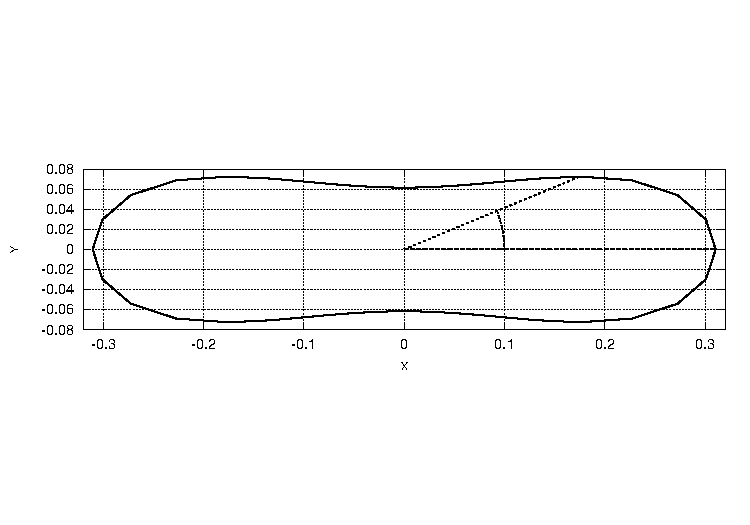
\includegraphics[width=\textwidth]{figures/orbit_theta_sup_1}
\caption{Hamiltonian orbit when $I>I_c$ and $K_{2I}<
K < K_s$}
\label{f:orbit_theta_sup_1}
\end{center}
\end{figure}

\begin{figure}
\begin{center}
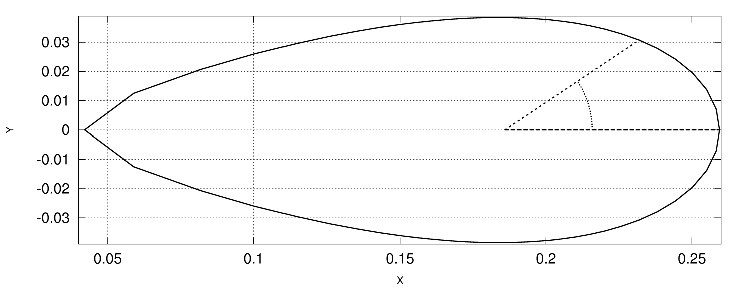
\includegraphics[width=\textwidth]{figures/orbit_theta_sup_2_cropped}
\caption{Hamiltonian orbit when $I>I_c$ and $K_s< K < K_e$}
\label{f:orbit_theta_sup_2}
\end{center}
\end{figure}

To apply~\eqref{e:polar integral}, $r(\theta)$ is calculated with a numerical root solver by transforming equation~\eqref{e:averaged K} to polar coordinates.

The procedure described above holds in the $K-I$ domain wherever the period is not infinite. The period is infinite along the edges $K_s$ and $\mathcal{K }_e$. Along the edge $K_s$ the diffusion coefficients have a finite value whereas the drift coefficients do not, but only the former need to be evaluated to impose the conservation of probability flux condition. Along the edge $\mathcal{K}_e$, the drift and diffusion coefficients are found by linearization about the coordinates of the elliptic fixed points. Sample representations of the drift and diffusion coefficients are shown in figure~\ref{f:drift diffusion figures}.

\begin{figure}
\begin{center}
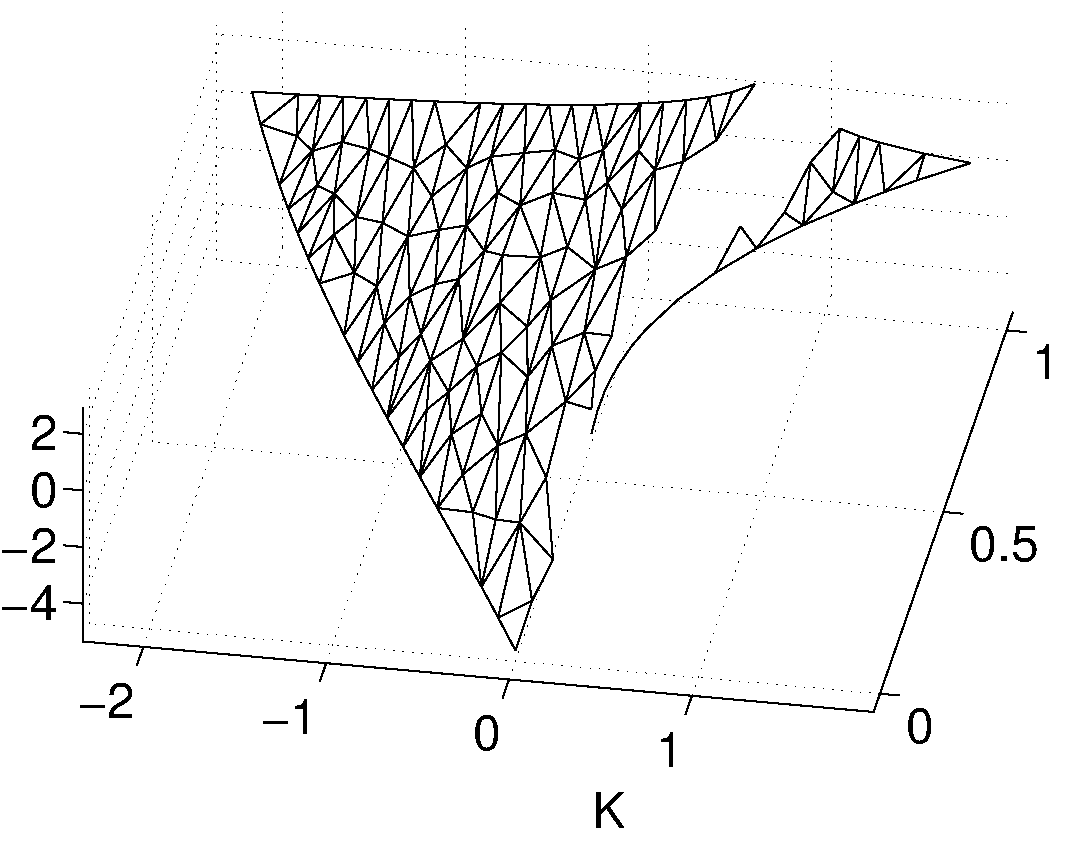
\includegraphics[width=\textwidth*7/16]{figures/b1_db4_mesh}
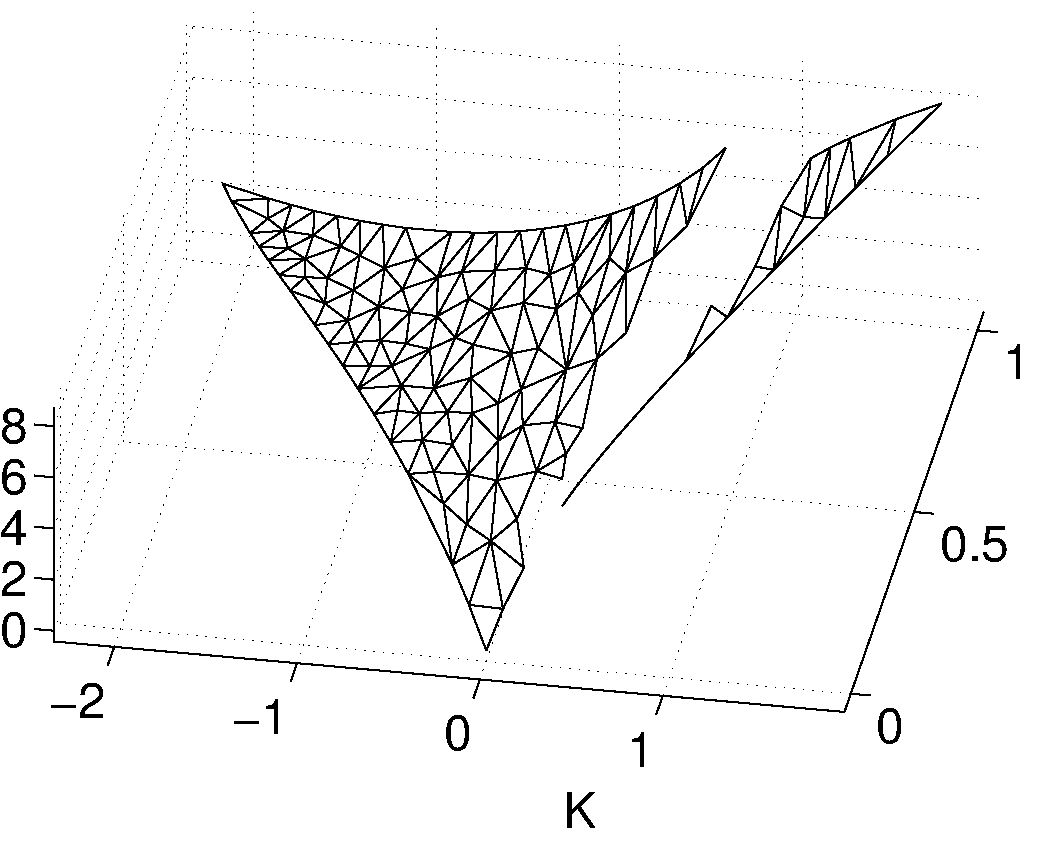
\includegraphics[width=\textwidth*7/16]{figures/a11_db4_mesh}
\caption{Drift $\mathring{\mathfrak b}_K$ (left) and diffusion $\mathring{\mathfrak a}_{\mathcal K \mathcal K}$ (right). Parameters are as follows: radius = 1, depth = 1, $\sigma_1 = -3$, $\sigma_2 = 0$, $\alpha_{1,2} = -0.25$, $\omega \mathcal{F}_c(\omega) = 25$}
\label{f:drift diffusion figures}
\end{center}
\end{figure}

\section{Conclusions}

In this chapter, it has been demonstrated that surface wave motion can be analyzed using stochastic averaging techniques. To achieve this a Hamiltonian model of surface wave motion was used to transform a set of governing partial differential equations into an infinite system of ordinary differential equations. Stochastic effects were then added to the model. Resonance was introduced and the geometry of the reduced graph of the stochastic process was established. Finally the averaged drift and diffusion coefficients were calculated throughout the domain. To do so, numerical algorithms were devised and special care was given to the boundaries of the reduced graph where singularities can manifest themselves.

With the drift and diffusion coefficients determined, a two-dimensional reduced Markov process has been characterized in the weak sense. In Chapter \ref{c:pdf}, our analysis continues. We will determine stationary probability density distributions associated with the generator of the surface waves problem.

% FIXME Freidlin's work suggests drift coefficient can be calculated along gluing edge

% FIXME Calculation at center edge _and_ I_c

% % Old Section
% To perform this quadrature, spatial averaging must be performed. First
% the orbits shown in Figures~\ref{f:X Y phase portrait I < I_c}
% and~\ref{f:X Y phase portrait} need to be computed with some
% accuracy. These orbits can be obtained in at least two ways. The first
% is to solve the equations for $\dot{X}_t$ and $\dot{Y}_t$
% (Equations~\eqref{e:Xdot} and~\eqref{e:Ydot}) as a set of ODEs,
% the second method is to calculate contour levels of the
% Hamiltonian. We do the latter using MATLAB's \emph{contourc}
% function. With this method, in order to maintain approximately the
% same accuracy throughout the domain $\mathfrak{G}$, it appears that
% the number of gridpoints on which $K$ is calculated and used
% as input to the function \emph{contourc} must be approximately the
% same for all orbits.
%
% \emph{Contourc} outputs a list of $X,Y$ coordinates at which
% $K$ has a specified value thus making it possible to
% calculate $\mathfrak{b}_i$ and $\mathfrak{a}_{jk}$.
